\section{Dual View: New Insights on Prior Result and New Results}\label{sec:analysis}
 %We continue to be in the DGN setting of characterising learning the weights with fixed gates in the limit of infinite width as in \Cref{sec:fixedgates}. We already saw that this setting is characterised by the NPK. 
In this section is to present new theoretical insights on prior result and new theoretical results with insights to justify the claim that the learning of the weights given the gates is \emph{disentangled in the path space}. By this, we mean that it is enough to think that the value network is dual linear, i.e., it simply computes/learns the inner product $\hat{y}_{\text{DGN}}=\ip{\phi_{\Tf}(x),v_{\Tv}}$. There are two compelling reasons to adopt the dual view. Reason-(i): In \Cref{sec:gatelearning} we saw that the fixed learnt gates ($79.68\%$) recover almost all the performance of the DNN ($80.32\%$), i.e., dual linearity is not a mere conceptualisation, but is analogous to a linear model in practice as well. In other words, just like one can learn weight vector in a linear model given the features, one can learn the neural path value given the neural path features. Reason-(ii): in the fixed gates infinite width setting, we  already have an interpretation via the NPK.

The conceptual issue that stops us from adopting the dual view is the commonly held view that `sophisticated features are learnt in a layer-by-layer' manner. That is, in a DGN, given that the input $x\in\R^{\din}$  is presented to the value network, it could be argued that the GaLUs and linear operations are entangled which in turn enable learning of sophisticated features in the layers. To demystify the layer-by-layer processing viewpoint, in the DGN and DLGN the value network can be provided with a constant $\mathbf{1}$. This is to show that if the input $x\in\R^{\din}$ is not given to the value network in the first place it is not possible to learn sophisticated structures in a layer-by-layer manner. In terms of the dual linearity, providing a constant $\mathbf{1}$ input has only a minor impact, in that, the neural path feature becomes $\phi(x,p)=1\cdot A(x,p)$, i.e., it still encodes the path activity which is still input dependent. Since $\phi(x)$ depends only on gates, the NPK will depend only on the $\textbf{overlap}$ matrix; all the theoretical results in this section will capture the effect. Now, it could be argued that, despite a constant $\mathbf{1}$ input, the gates are still arranged layer-by-layer, due to which, the network is able to still learn sophisticated structures in a layer-by-layer manner. All the results in this section will point out that as long as the \textbf{correlation of the gates} is not lost, the layer-by-layer structure can be destroyed.

We now present new insights on Theorem 5.1 in \citep{npk} (as in \Cref{th:fcprev}) by restating it explicitly in terms of the gates in \Cref{th:fc}. The prior work in dual view was for fully connected networks. Here, we extend the dual view to reveal additional structure of the NPK in the presence of convolutions with global-average-pooling and skip connections in \Cref{th:conv,th:res} respectively and discuss the new insights by comparing with related work.
%In what follows, we first restate the prior result. While \Cref{th:fc} and Theorem 5.1 in \citep{npk} are mathematically identical, \Cref{th:fc} is written in a manner to capture the fact that the NPK is invariant to permutation of the layers. \Cref{th:conv,th:res} are entirely new and are extensions of the dual view for convolutions with global pooling and skip connections. 


%\subsection{NPK of FC-DNN: Product Kernel }
%\input{cnpkexample}
%\subsection{Neural Path Kernel : Similarity based on active sub-networks}
%\textbf{Remark.} In the case of fully connected networks, $\textbf{overlap}_{\Theta}(i,x,x')$ is equal for all $i\in[\din]$, and hence $\text{NPK}_{\Theta}(x,x')=\ip{x,x'}\cdot\textbf{overlap}_{\Theta}(x,x')$.
%We point out that this statistical decoupling of weights and gates in \Cref{assmp:main} is unrealisable in a DNN with ReLU, however, this assumption can be trivially realised in a DGN. %Further, we are interested only in the `what?' ( and not `how?') question related to the gates in which case this assumptions is not a restriction.
\subsection{Fully Connected: New Insights on Prior Result}
\begin{theorem}[Product of Kernels Theorem]
\label{th:fc} Let $G_l(x)\in[0,1]^w$ denote the gates in layer $l\in\{1,\ldots,d-1\}$ for input $x\in\R^{\din}$. Under \Cref{assmp:main}  ($\sigma=\frac{\cscale}{\sqrt{w}}$) for FC-DGN : 
\begin{align*}
\text{NTK}(x,x') \rightarrow d \cdot \cscale^{2(d-1)} \cdot \left(\ip{ x,x'} \cdot \Pi_{l=1}^{d-1} \frac{\ip{G_l(x),G_l(x')}}w\right), \quad\text{as}\,\, w\rightarrow \infty 
\end{align*}
\end{theorem} 
$\bullet$ \textbf{Product Kernel : Role of Depth and Width.} \Cref{th:fc} is mathematically equivalent to Theorem 5.1 in \citep{npk} (stated as \Cref{th:fcprev}). The equivalence follows from the simple observation that $\textbf{overlap}(x,x')=\Pi_{l=1}^{(d-1)}\ip{G_l(x),G_l(x')}$. While this observation is very elementary in itself, it is significant at the same time;  \Cref{th:fc} provides the most simplest kernel expression that characterises the information in the gates. It also explains the roles of width and depth.  From \Cref{th:fc} it is evident that the role of width is \emph{averaging} (due to the division by $w$). Each layer therefore corresponds to a \emph{base kernel} $\frac{\ip{G_l(x),G_l(x')}}w$ which measures the \emph{\textbf{correlation of the gates}}. The role of depth is to provide the product of kernels. To elaborate, the feature network provides the gates $G_l(x)$, and the value network implements the product kernel in \Cref{th:fc} by laying out the gates as masks depth-wise, and connecting them in the structure of a deep network. Note that depth-wise layout plays an important role here: for instance, if we were to concatenate the gating features as $\varphi(x)=(G_l(x),l=1,\ldots,d-1)\in\{0,1\}^{(d-1)w}$, it would have only resulted in the kernel $\ip{\varphi(x),\varphi(x')}=\sum_{l=1}^{d-1}{\ip{G_l(x),G_l(x')}}$, i.e., a \emph{sum  (not product)} of kernels. 

$\bullet$ \textbf{Constant $\mathbf{1}$ Input.} This has a minor impact in that the expression on right hand side of \Cref{th:fc} becomes $d \cdot \cscale^{2(d-1)} \cdot \din \cdot \Pi_{l=1}^{d-1} \frac{\ip{G_l(x),G_l(x')}}w$, i.e., the kernel still has information of the gates.

$\bullet$ \textbf{Destroying structure by permuting the layers.}  $\Pi_{l=1}^{d-1} \frac{\ip{G_l(x),G_l(x')}}w$ is permutation invariant, and hence permuting the layers has no effect.


%\textbf{Remark.} Here $\frac{\ip{G_l(x),G_l(x')}}w$ are the \emph{base kernels} measuring the \emph{\textbf{correlation of the gates}}. We show experimentally that the correlation of gates is essentially  `what is learnt in a DNN with ReLUs'.
%and $\Pi_{l=1}^{d-1} \frac{\ip{G_l(x),G_l(x')}}w$ is a product of these base kernels and hence the name `Product of Kernels Theorem'.  The base kernels are essentially measuring which we show via  We now list the roles of the two networks, weights, depth and width.

%\textbf{Feature Network.} The role of this network is to process the input layer-by-layer and produce the $w$-dimensional gating features $G_l(\cdot)$. Each layer comprises of `$w$' ReLUs, and a given ReLU (i.e., gate) is `on' if the input to that layer lies on the positive half-space of hyperplane of given by the incoming weights of that ReLU. Thus the gates of a given layer are based on the angle between the input to that layer and the various hyperplanes given by the weights of that layer. Prior experiments in [\citenum{npk}] and the experiments in this paper show that the feature network, i.e., the gates hold most information, which in turn means that weights of the feature network are key.

%\textbf{Value Network}. The value network implements the product of kernels by laying out the gates as masks depth-wise, and connecting them in the structure of a DNN. Note that depth-wise layout plays an important role here: for instance, if we were to concatenate the gating features as $\varphi(x)=(G_l(x),l=1,\ldots,d-1)\in\{0,1\}^{(d-1)w}$, it would have only resulted in the kernel $\ip{\varphi(x),\varphi(x')}=\sum_{l=1}^{d-1}{\ip{G_l(x),G_l(x')}}$, i.e., a \emph{sum  (not product)} of kernels. Prior experiments in [\citenum{npk}] and the experiments in this paper show that the value network can be reset and re-trained without loss of performance, which in turn means that weights of the value network are not that important.

%\textbf{Note.} The above insights from \Cref{th:main} carry over to the case of DNN with ReLUs by thinking that the roles of value and feature network are performed by a single network.
\subsection{Convolution  Global Average Pooling: New Result I}
Let the circular rotation of vector $x\in\R^{\din}$ by `$r$' co-ordinates be defined as $rot(x,r)(i)=x(i+ r)$, if $i+r \leq \din$ and $rot(x,r)(i)=x(i+ r-\din)$ if $i+r > \din$.  The architecture and the notations for the network with convolutions is presented in the Appendix. %Using circular convolutions with pooling results in a rotationally invariant kernel \Cref{th:mainconv}.
\begin{comment}
 We extend the dual view to neural network with $\dc$ convolutional layers ($l=1,\ldots,\dc$), followed by a \emph{global-average/max-pooling} layer ($l=\dc+1$) and $\dfc$ ($l=\dc+2,\ldots,\dc+\dfc+1$) fully connected  layers (see Appendix for notation). The convolutional window size is $\wconv<\din$, the number of filters per convolutional layer as well as the width of the fully connected layers is $w$. The main steps are (i) treating pooling layers like gates/masks, (ii) bundling together the paths that share the same path value (due to weight sharing in convolutions) and (iii) re-defining the NPF and NPV for these bundles. The important consequence of weight sharing (due to convolutions and pooling) is that the NPK becomes rotationally invariant resulting in \Cref{th:mainconv}.
\end{comment}
\begin{theorem}[Rotationally Invariant Kernel Theorem]\label{th:conv} Under \Cref{assmp:main}, for  a suitable $\bcnn$:
\begin{align*}
\text{NTK}(x,x')\rightarrow  \frac{\bcnn}{{\din}^2} \cdot \sum_{r=0}^{\din-1} \ip{x,rot(x',r)}_{\textbf{overlap}(\cdot, x,rot(x',r))},\,\, \text{as}\,\,  w\rightarrow\infty\,
\end{align*}
\end{theorem}

$\bullet$ The constant $\bcnn$ in \Cref{th:conv} is expanded in the appendix.

$\bullet$ $\sum_{r=0}^{\din-1} \ip{x,rot(x',r)}_{\textbf{overlap}(\cdot, x,rot(x',r))}=\sum_{r=0}^{\din-1}\sum_{i=1}^{\din} x(i) rot(x',r)(i)\textbf{overlap}(i,x,rot(x',r))$, where the inner `$\Sigma$' is the inner product between $x$ and $rot(x',r)$ weighted by $\textbf{overlap}$ and the outer `$\Sigma$' covers all possible rotations, which in addition to the fact that the all the variables internal to the network rotate as the input rotates, results in the rotational invariance property.  .It was observed in the experiments of \cite{arora2019exact} that networks with global-average-pooling are better than vanilla convolutional networks. The rotational invariance property holds for architectures using convolutional layer only in the presence of global-pooling.  So, this result explains why global-average-pooling helps. That said, this rotational invariance property of the kernel is not a new observation in this paper; it was shown by \cite{li2019enhanced} that  prediction using CNTK-GAP is equivalent to prediction using CNTK without GAP but with full translation data augmentation  (this same as rotational invariance) with wrap-around at the boundary  (this same as circular convolution). However, \Cref{th:conv} is a necessary result for the dual view, in that, it demonstrates that this rotational invariance property is recovered in the dual view as well. 

$\bullet$ In \Cref{th:conv} the expression becomes $\frac{\bcnn}{{\din}^2} \cdot \sum_{r=0}^{\din-1}\sum_{i=1}^{\din} \textbf{overlap}(i,x,rot(x',r))$ for a  \textbf{constant $\mathbf{1}$ input}. The key novel insight is that the rotational invariance is not lost and the kernel still encodes the correlation in the gates via the $\textbf{overlap}$ matrix which measures the correlation of the paths.

$\bullet$ \textbf{Destroying structure by permuting the layers} does not destroy the rotational invariance property of the expression in \Cref{th:conv}. This is because due to circular convolutions throughout all the variables internal to the network rotate as the input rotates. Permuting the layers, only affects the ordering in which the gates appear, and does not affect the fact that the gates rotate as the input rotates.

\subsection{Residual Networks With Skip Connections (ResNet): New Result II}
We consider a ResNet with `$(b+2)$' blocks and `$b$' skip connections between the blocks. Each block is a fully connected (FC) network of depth `$\dblock$' and width `$w$'. There are $2^b$ many sub-FCNs within this ResNet (see \Cref{def:subfcdnn}).
Also note that the blocks being fully connected is solely for expository purposes, and the results hold even if the blocks are convolutional networks instead.

%and right of \Cref{fig:resnet}).
%\FloatBarrier
\begin{comment}
\begin{figure}[t]
\begin{minipage}{0.5\columnwidth}
\resizebox{\columnwidth}{!}{
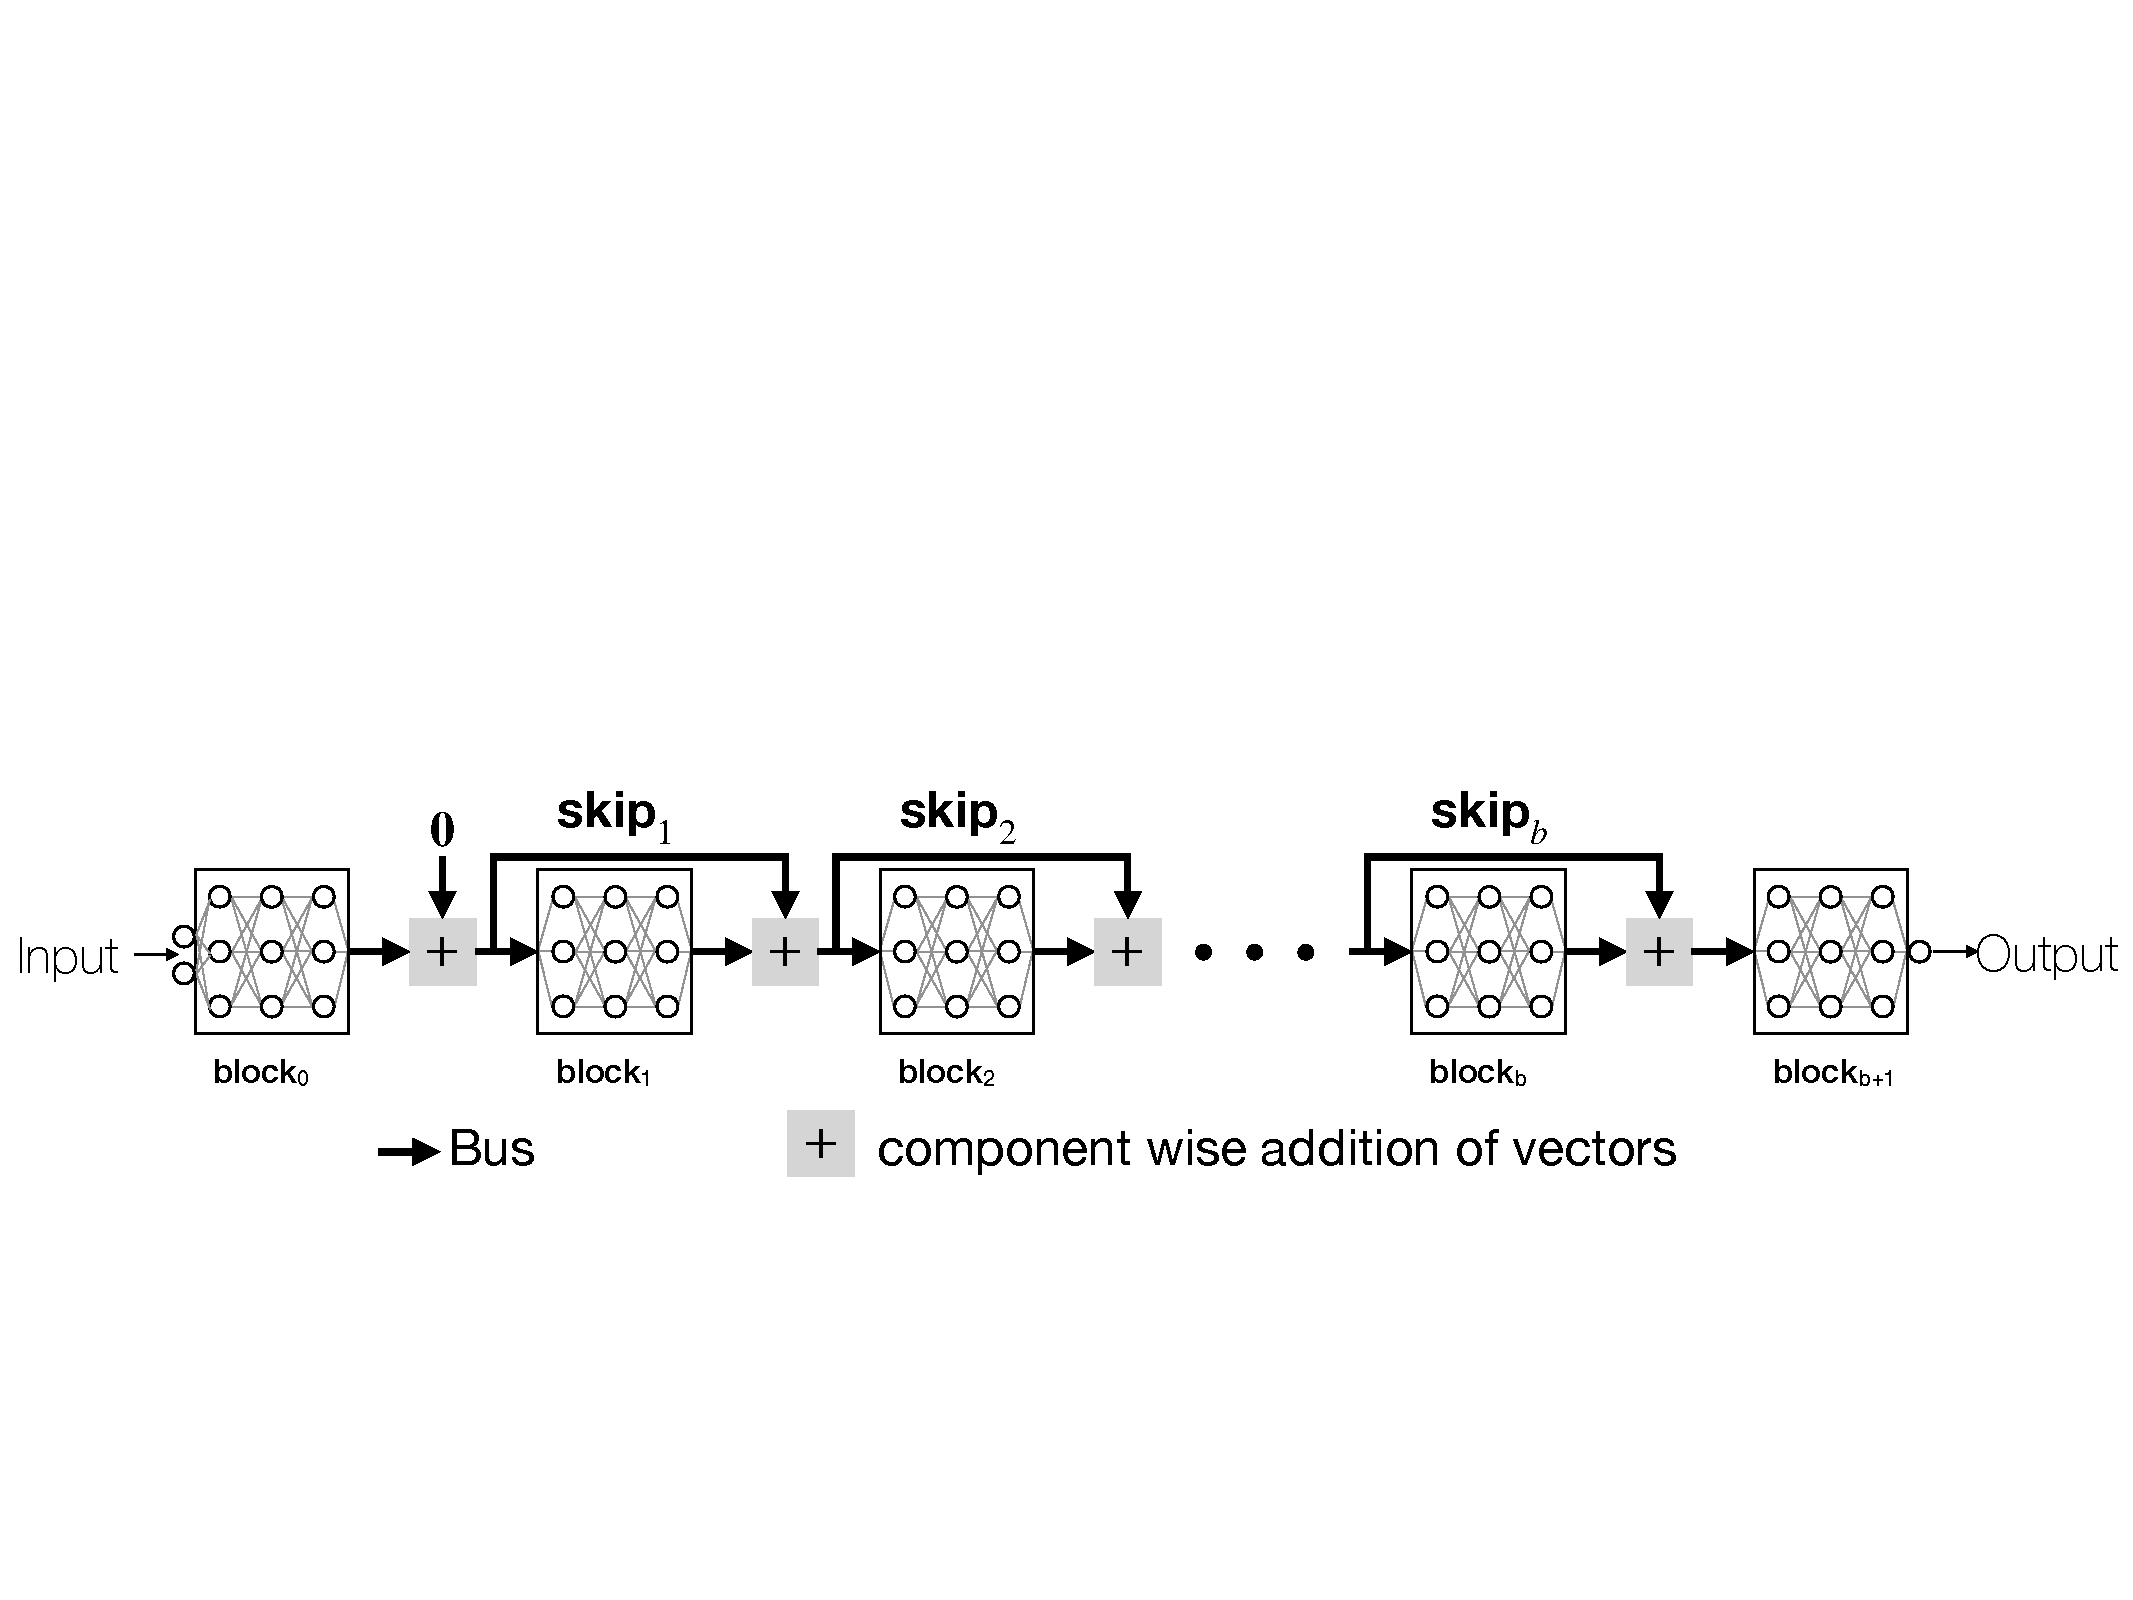
\includegraphics[scale=0.5]{figs/resnet.pdf}
}
\end{minipage}
\begin{minipage}{0.5\columnwidth}
\resizebox{\columnwidth}{!}{
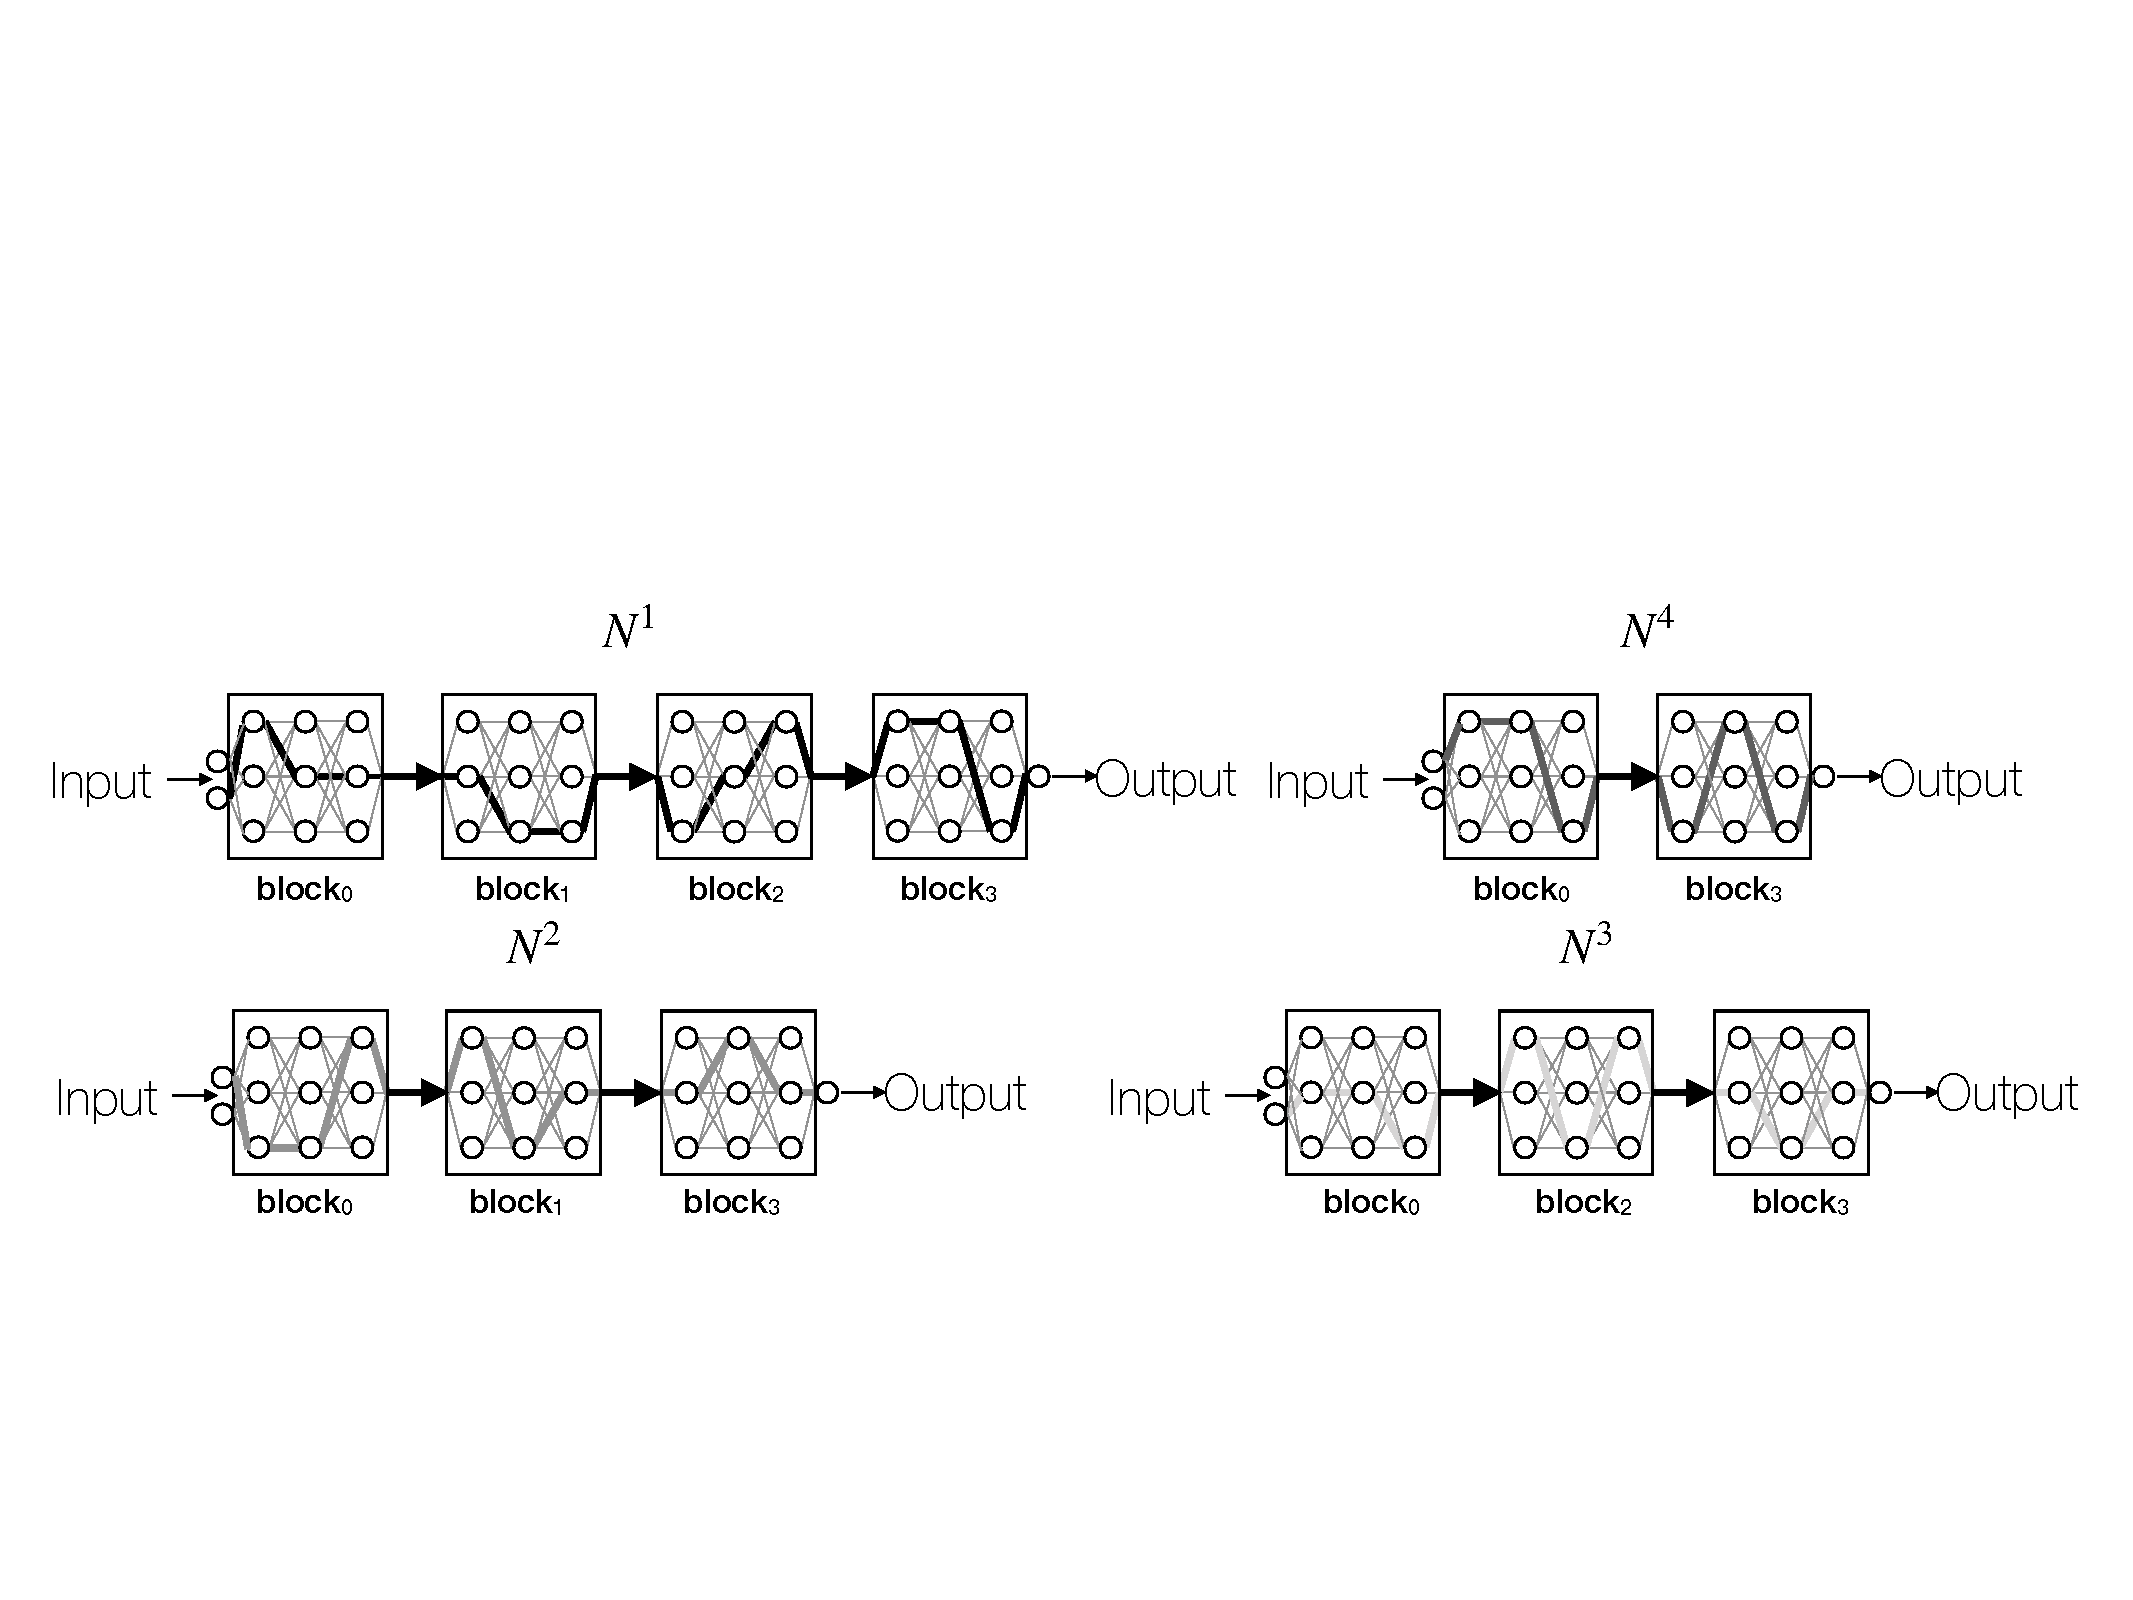
\includegraphics[scale=0.5]{figs/blocks.pdf}
}
\end{minipage}
\caption{\small{Figure on the left is the ResNet with $b$ skip connections and $(b+2)$ blocks. Figure on the right shows for $b=2$, the sub-FCNs $N^1$ obtained by skipping no blocks, $N^2$ and $N^4$ obtained by skipping block $1$ and $2$ respectively, and $N^3$ obtained by skipping both blocks $1$ and $2$.}}
\label{fig:resnet}
\end{figure}
\end{comment}
\begin{definition}\label{def:subfcdnn}[Sub FC-DNNs]
Let $2^{[b]}$ denote the power set of $[b]$ and let $\J\in 2^{[b]}$ denote any subset of $[b]$. Define the`$\J^{th}$' sub-FCN of the ResNet to be the fully connected network obtained by (i) including  $\text{block}_{j},\forall j\in \J$  and (ii) ignoring $\text{block}_{j},\forall j\notin \J$. %(see \Cref{fig:resnet}).
\end{definition}
\begin{theorem}
[Ensemble Of Kernels Theorem]\label{th:res} Let $\text{NPK}^{\J}$ be the NPK of the $\J^{th}$ sub-FCN, and $\bfc^{\J}$ be the associated constant. Under \Cref{assmp:main}, we have:
\begin{align*}
\text{NTK}\rightarrow \sum_{\J\in 2^{[b]}}  \bfc^{\J} \text{NPK}^{\J}, \,\, \text{as}\,\,  w\rightarrow\infty
\end{align*}
\end{theorem}
%\textbf{Note.} The sub-FC-DNNs we refer to in \Cref{th:mainres} belong to (or are parts of) the feature network from which the gates are obtained. 

$\bullet$ The constant $\bfc^{\J}$ is expanded in the Appendix. 

$\bullet$ \textbf{Ensemble.} To the best of our knowledge, this is the first theoretical result to show that ResNets have an ensemble structure, where  each kernel in the ensemble, i.e., $\text{NPK}^{\J}$ corresponds to one of the $2^b$ sub-architectures (see \Cref{def:subfcdnn}). The ensemble behaviour of ResNet and  presence of $2^b$ architectures was observed by \cite{veit2016residual}, however without any concrete theoretical formalism. 

$\bullet$ The effect of \textbf{constant $\mathbf{1}$ input} continues to hold to all the kernels (which are fully connected networks themselves) in the ensemble and hence to the overall kernel.

$\bullet$ \textbf{Destroying structure} \cite{veit2016residual} showed empirically that ``removing single layers from residual networks at test time does not noticeably affect their performance", and yet ``removing a layer from a traditional architecture such as VGG leads to a dramatic loss in performance". \Cref{th:res} can be seen to provide a theoretical justification for this empirical result. In other words, due to the ensemble structure a ResNet is capable of dealing with failure of components. While, failure of component itself does not occur unless one makes them fail purposefully in experiments as done in \citep{veit2016residual},  the insight is that even if one or many of the kernels in the ensemble are corrupt and the good ones can compensate for them. 
%The main novelty in our paper compared to \citep{veit2016residual} is that we provide a mathematical framework and also the expression for the ensemble kernel. Thus, our results are theoretical and \citep{veit2016residual} presents empirical results without rigorous theory.

%In order to completely address the `black box'-ness issue, an ideal goal is to aim for theoretical results (supported by empirical evidence) on finite time learning in finite width \texttt{DGN-NO-ACT}. We find this goal is too hard at this stage and do not pursue the same. The next level is to analyse  the primal linearity and the dual linearity separately. Understanding the primal linearity has two parts to it (i) `what do the learnt pre-activations mean?', and (ii) `how are useful pre-activations learnt?'. The `what' question is \emph{post-hoc}, i.e., we can inspect the learnt pre-activations after training. However, we believe that in order to obtain domain specific insights on what the learnt pre-activations mean, we might require domain specific tools. For instance, in the case of `image classification', the pre-activations are the result of series of convolutions by `filter banks', and in order to do full justice, any visual interpretation should also tally with the results from `filter bank' theory. We defer the `what' question for future work. We also believe new theory is required to answer `how are useful pre-activations learnt?', and defer the same to future work. In this paper,  


%$\bullet$ We empirically show that \texttt{DGN-NO-ACT} performs comparably well on standard datasets. 

%$\bullet$ We restate the prior result for the fully connected case so as to explicitise the role of gates, depth and width. We extend the dual view theory to cover  convolutions with global pooling and skip connections.  We show empirically that the value network learns path-by-path and not layer-by-layer.




%A \texttt{DGN-NO-ACT} learns the relation $\hat{y}(x)=\ip{\phi_\Tf(x),v_{\Tv}}$, by learning simultaneously the feature and value network parameters. The pre-activations generated by the feature network trigger the gates thereby directly dictating the neural path feature $\phi_\Tf(x)$. It was shown that neural path features (i.e., the gates) are learnt during training and such learning improves generalisation \cite{npk}. Thus, while the learning in feature network is key, we reserve its theoretical study for future work. In this section, we will analyse the dual linearity, wherein, the theoretical results are in the \emph{inifinite width regime} which yield us a \emph{kernel} interperation, using which we probe into the properties of finite width networks. In other words, our aim is not to propose pure kernel methods with the kernel derived from an inifnite width DNN. 

%For the purpose of analysing the dual, we first explicitise in \Cref{th:fc} an unnoticed invariance property in the prior result of \cite{npk} for fully connected networks. In \Cref{th:conv,th:res} we also extend the dual formulation to cover the cases of convolutions with global pooling and skip connections. These results justify the constant $\mathbf{1}$ input to the value network of the \texttt{DGN-NO-ACT}. We also experimentally verify the constant $\mathbf{1}$ input as well as destroying the layer-by-layer structure of the gates does not degrade the performance. While these results are surprising and counter intuitive with respect to the primal view, they are follow in a straightforward manner from the results in the dual view, thereby underscoring the fact the value network indeeed computes path-by-path, and eliminating the `mystery' as to whether sophisticated structures are learnt layer-by-layer.

